% Source PDF pp. 40-46 / standard pp. 28-34.
% Continues 4.2.1, completes 4.2 and 4.3, and begins 4.4.

% ---------------------------------------------------------------------------
% Source PDF p. 40 / standard p. 28.
% ---------------------------------------------------------------------------
\newpage
Object classes provide the means for federation participants to subscribe to information about all individual instances of HLA objects with common characteristics, such as all sports cars or all fighter jets. Classes are also essential to specifying characteristics (attributes) of simulation objects, because these are defined relative to classes of objects, not unique to individual instances. In addition, because basic HLA services (as described in IEEE Std 1516.1-2010) support subscriptions to object class attributes by federates participating in a federation execution, the RTI requires knowledge of all object classes and their attributes if it is to support distribution of HLA object information by class to the federates of a federation execution.

A class hierarchy expands the capabilities of a flat classification scheme by enabling federates to subscribe to information about broad superclasses of objects, such as all ground vehicles, all air vehicles, or all sea vehicles. IEEE Std 1516.1-2010 supports subscription to attributes of any class in an object class hierarchy so that federates can easily subscribe to attributes of all or only those classes of interest. An object class hierarchy also supports simplification of the specification of attributes by placing common attributes of multiple subclasses in a common superclass. Thus, class hierarchies enable simpler management of the interests of different federates in the objects and attributes involved in a federation execution.

\subsubsection{Table format}
The object class structure template of Table 4 provides a format for representing the class-subclass hierarchy of object classes. It shall be populated by first entering the root class of all object classes in the left-most column; this object class is named ``HLAobjectRoot.'' Then, the most general object classes shall be entered in the next column, followed by all of their immediate subclasses in the next column, and then further levels of subclasses, as required. The number of intermediate columns used depends on the needs of the federate or federation. A federate or federation that uses a deeper hierarchy than illustrated by the template of the table shall add columns as needed. Finally, the most specific object classes shall be specified in the right-most column. Object class names shall adhere to HLA naming conventions (see 3.3.1).

Although individual class names need not be unique, all object classes shall be uniquely identifiable in an HLA object model when concatenated (via dot notation) with the names of higher-level superclasses.

Each object class in the object class structure table shall be followed by information on publication and subscription capabilities enclosed in parentheses, as designated in the template using the abbreviated variable name \omtph{p/s}.

% ---------------------------------------------------------------------------
% Source PDF p. 41 / standard p. 29.
% ---------------------------------------------------------------------------
\newpage
For a SOM or SOM module, valid entries for \omtph{p/s} shall be as follows:
\begin{itemize}[leftmargin=32pt,labelwidth=10pt,labelsep=12pt,itemsep=2pt,topsep=2pt]
\item \textit{P (Publish):} The federate is capable of publishing at least one attribute of the object class.
\item \textit{S (Subscribe):} The federate is capable of subscribing to at least one attribute of the object class.
\item \textit{PS (PublishSubscribe):} The federate is capable of publishing at least one attribute and subscribing to at least one attribute of the object class.
\item \textit{N (Neither):} The federate is incapable of either publishing or subscribing to any attributes of the object class.
\end{itemize}

For a FOM or FOM module, the same entries for \omtph{p/s} are valid. However, an object class is classified as Publish or Subscribe in the federation if at least one federate is capable of publishing or subscribing to at least one attribute in the context of the object class.

Classes designated as Subscribe or Neither can have no registered instances, but they can have subclasses that can be registered.

\vspace{10pt}
\omtcaption{Table 4---Object class structure table}
\vspace{-7pt}
\omtclassstructuretemplate{HLAobject Root}{(\omtph{p/s})}{1.024}

\vspace{8pt}

\subsubsection{Inclusion criteria}
\vspace{4pt}
In all HLA object models, any object class that is referenced in any table within the object model shall also be included in the object class hierarchy. The criteria for designing an object class hierarchy for an HLA object model is fundamentally different for individual federates than for federations. The object class structure table of a FOM or FOM module represents an agreement between the federates in a federation on how to classify object classes for the purposes of federation executions. The object class structure table of a SOM or SOM module is a type of advertisement of the classes of objects that the federate can support (as Publish or Subscribe) in potential federations. In neither case does the HLA require specific object classes (other than the required root class) or object class hierarchies to appear in the object class structure table.

% ---------------------------------------------------------------------------
% Source PDF p. 42 / standard p. 30.
% ---------------------------------------------------------------------------
\newpage
For individual federates, it is the intrinsic functionality (expressed as classes of objects) that the federate can offer to future HLA federations---and any object classes whose instances (and associated instance attribute values) may potentially represent useful information if generated by other HLA federates---that defines the content of the object class structure table. The structure of the object class hierarchy is driven by how the federate supports class publication and subscription. Rich, deep SOM class hierarchies can provide federates with a significant degree of flexibility in how they can support and participate in federations in the future.

For federations, it is the subscription requirements of the collective set of simulations participating in the federation that drives the content and structure of the object class hierarchy. Although a set of object classes for the most specific types of entities involved in a federation (e.g., cruiser, refrigerator) may completely satisfy the subscription requirements of some types of HLA applications, additional higher-level object classes would be needed if federates wish to be able to subscribe to HLA object information at higher levels of abstraction (e.g., navy surface ships, kitchen appliances). For a federate to be able to subscribe to HLA object information at a desired level of abstraction, an object class at that level of abstraction shall appear in the object class structure table.

For example, suppose a federation involved air, land, and sea forces of many specific types. If a particular federate did not require notification of the specific types of land vehicles, but did require notification of land vehicles in its area of interest, a suitable class (such as GroundVehicle) that contained specific vehicle types as subclasses would be needed to make this possible.

Although classes are clearly needed for all objects of interest in a federation, many alternative class hierarchies can be devised to cover any given set of objects. The demarcations and levels of classes selected for an HLA FOM are the result of the federation development process. Object class hierarchies that already exist for individual FOM modules, SOM modules, and SOMs may be incorporated into a FOM object class hierarchy if they meet the interests of the federation as a whole.

\subsubsection{Example}
Table 5 provides an example of how the object class structure table can be used to represent a simple system. In this case, the system being represented is a typical neighborhood restaurant. The simulation of this restaurant's operations can be considered to be a potential federate in a larger scale federation, perhaps representing the combined, coordinated operation of a chain of restaurants. The intent of this example is not to specify a complete SOM for this system, but rather to provide partial illustrations of how the OMT tables can be used to capture relevant information about the system.

In this example, a subset of a complete object class hierarchy is shown as consisting of five object classes at the most general level. For this simulation, no class decomposition was necessary for the first three classes. For the fourth class, a single level of decomposition is shown resulting in five leaf classes. For the fifth class, several levels of decomposition are shown to illustrate a partial representation of the restaurant's menu. Some of the deeper levels in this hierarchy could have been modeled as attributes (e.g., ClamChowder could have been a leaf class, with an attribute of Type to represent the enumerated values of Manhattan or NewEngland). However, the modeler in this example opted to represent the most specific food types as individual classes.

In this example, most nonleaf classes are designated as Subscribe only, whereas the leaf classes are designated as both Publish and Subscribe. One exception to this is the Employee class, which contains several attributes that are only published or subscribed to at the subclass level. Another exception is the ClamChowder class, which provides an example of a nonleaf class that can be registered (i.e., has attributes that can be published for that class). Finally, Manhattan and NewEngland provide examples of publishable leaf classes that do not contain subscribable attributes.

% ---------------------------------------------------------------------------
% Source PDF p. 43 / standard p. 31.
% ---------------------------------------------------------------------------
\newpage
\omtcaption{Table 5---Object class structure table example}
\vspace{-9pt}
\noindent\makebox[\textwidth][c]{%
    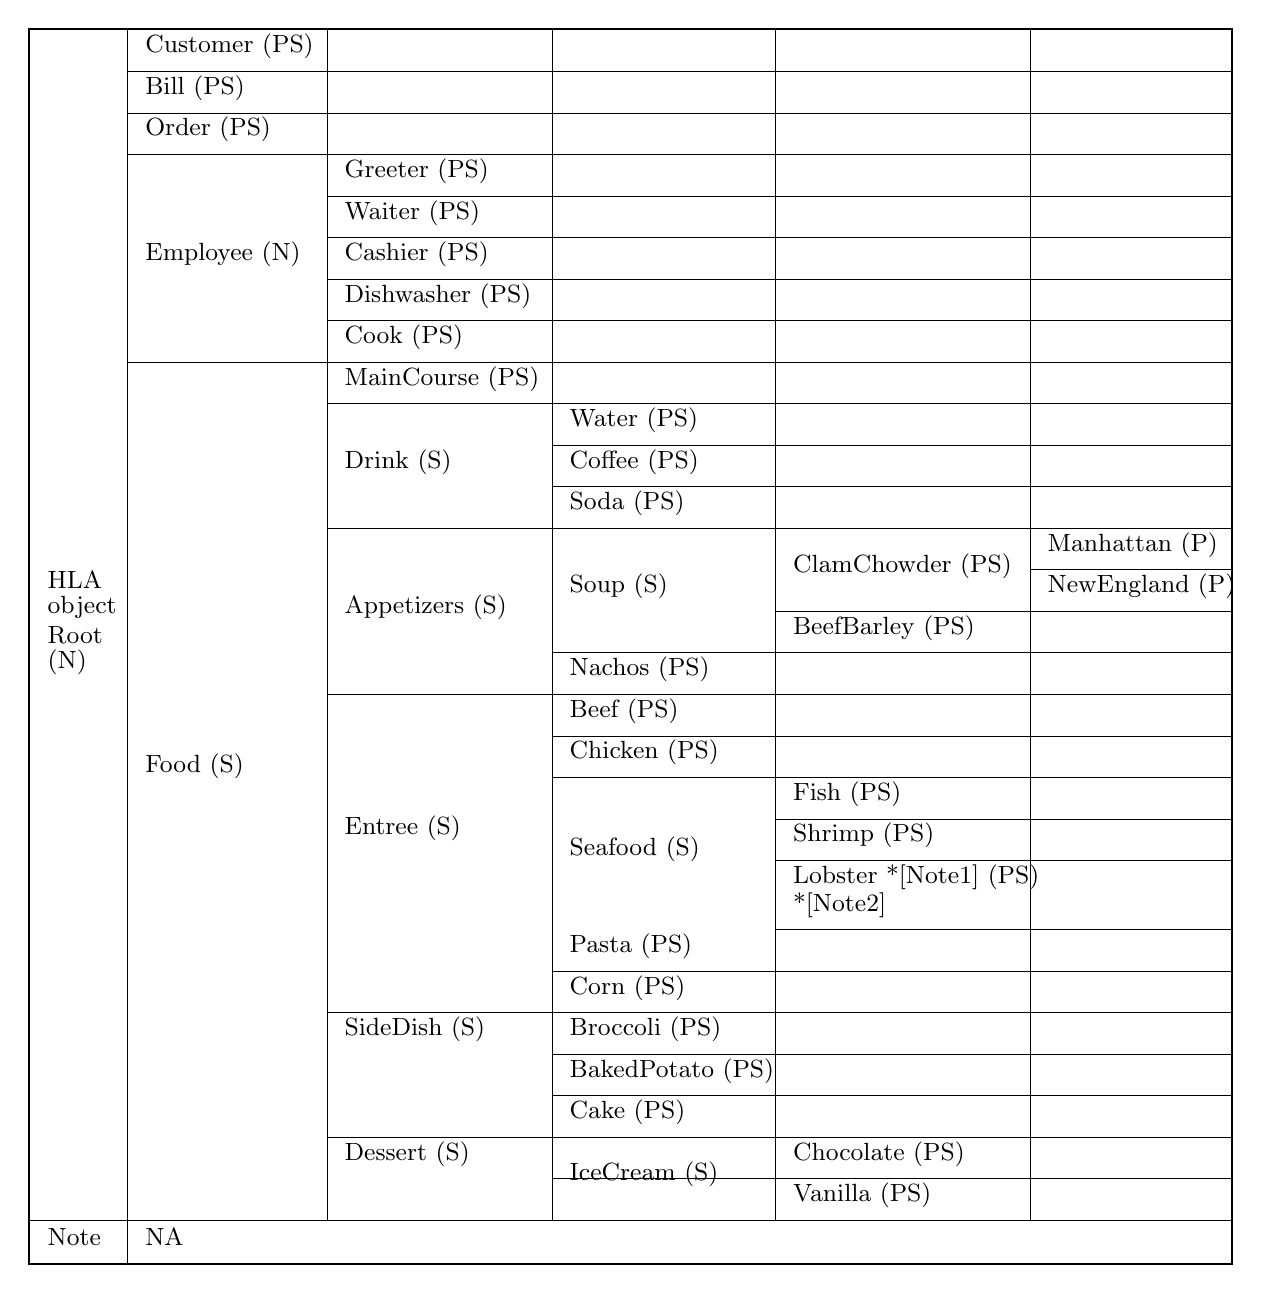
\begin{tikzpicture}[x=1pt,y=-1pt]
        \tikzset{omt5/.style={anchor=west,inner sep=0pt,font=\fontsize{9}{10}\selectfont}}
        % Frame and hierarchy columns, measured from the source table.
        \draw[line width=0.75pt] (0,0) rectangle (434.64,446.28);
        \draw[line width=0.28pt] (35.82,0)--(35.82,446.28);
        \draw[line width=0.28pt] (107.82,0)--(107.82,430.50);
        \draw[line width=0.28pt] (189.18,0)--(189.18,430.50);
        \draw[line width=0.28pt] (269.88,0)--(269.88,430.50);
        \draw[line width=0.28pt] (361.86,0)--(361.86,430.50);

        % Row boundaries; line starts encode the merged hierarchy cells.
        \foreach \yy in {15.48,30.48,45.48} {\draw[line width=0.28pt] (35.82,\yy)--(434.64,\yy);}
        \foreach \yy in {60.54,75.54,90.54,105.54} {\draw[line width=0.28pt] (107.82,\yy)--(434.64,\yy);}
        \draw[line width=0.28pt] (35.82,120.54)--(434.64,120.54);
        \draw[line width=0.28pt] (107.82,135.54)--(434.64,135.54);
        \foreach \yy in {150.54,165.54} {\draw[line width=0.28pt] (189.18,\yy)--(434.64,\yy);}
        \draw[line width=0.28pt] (107.82,180.54)--(434.64,180.54);
        \draw[line width=0.28pt] (361.86,195.54)--(434.64,195.54);
        \draw[line width=0.28pt] (269.88,210.54)--(434.64,210.54);
        \draw[line width=0.28pt] (189.18,225.54)--(434.64,225.54);
        \draw[line width=0.28pt] (107.82,240.54)--(434.64,240.54);
        \foreach \yy in {255.54,270.54} {\draw[line width=0.28pt] (189.18,\yy)--(434.64,\yy);}
        \foreach \yy in {285.54,300.54} {\draw[line width=0.28pt] (269.88,\yy)--(434.64,\yy);}
        \draw[line width=0.28pt] (269.88,325.50)--(434.64,325.50);
        \draw[line width=0.28pt] (189.18,340.50)--(434.64,340.50);
        \draw[line width=0.28pt] (107.82,355.50)--(434.64,355.50);
        \foreach \yy in {370.50,385.50} {\draw[line width=0.28pt] (189.18,\yy)--(434.64,\yy);}
        \draw[line width=0.28pt] (107.82,400.50)--(434.64,400.50);
        \draw[line width=0.28pt] (189.18,415.50)--(434.64,415.50);
        \draw[line width=0.28pt] (269.88,430.50)--(434.64,430.50);
        \draw[line width=0.28pt] (0,430.50)--(434.64,430.50);

        % Root and first hierarchy level.
        \node[omt5] at (6.66,199.1) {HLA};
        \node[omt5] at (6.66,209.1) {object};
        \node[omt5] at (6.66,219.1) {Root};
        \node[omt5] at (6.66,229.1) {(N)};
        \node[omt5] at (41.94,6.5) {Customer (PS)};
        \node[omt5] at (41.94,21.5) {Bill (PS)};
        \node[omt5] at (41.94,36.5) {Order (PS)};
        \node[omt5] at (41.94,81.6) {Employee (N)};
        \node[omt5] at (41.94,266.6) {Food (S)};

        % Second hierarchy level.
        \node[omt5] at (113.94,51.6) {Greeter (PS)};
        \node[omt5] at (113.94,66.6) {Waiter (PS)};
        \node[omt5] at (113.94,81.6) {Cashier (PS)};
        \node[omt5] at (113.94,96.6) {Dishwasher (PS)};
        \node[omt5] at (113.94,111.6) {Cook (PS)};
        \node[omt5] at (113.94,126.6) {MainCourse (PS)};
        \node[omt5] at (113.94,156.6) {Drink (S)};
        \node[omt5] at (113.94,209.1) {Appetizers (S)};
        \node[omt5] at (113.94,289.1) {Entree (S)};
        \node[omt5] at (113.94,361.6) {SideDish (S)};
        \node[omt5] at (113.94,406.6) {Dessert (S)};

        % Third hierarchy level.
        \node[omt5] at (195.30,141.6) {Water (PS)};
        \node[omt5] at (195.30,156.6) {Coffee (PS)};
        \node[omt5] at (195.30,171.6) {Soda (PS)};
        \node[omt5] at (195.30,201.6) {Soup (S)};
        \node[omt5] at (195.30,231.6) {Nachos (PS)};
        \node[omt5] at (195.30,246.6) {Beef (PS)};
        \node[omt5] at (195.30,261.6) {Chicken (PS)};
        \node[omt5] at (195.30,296.6) {Seafood (S)};
        \node[omt5] at (195.30,331.6) {Pasta (PS)};
        \node[omt5] at (195.30,346.6) {Corn (PS)};
        \node[omt5] at (195.30,361.6) {Broccoli (PS)};
        \node[omt5] at (195.30,376.6) {BakedPotato (PS)};
        \node[omt5] at (195.30,391.6) {Cake (PS)};
        \node[omt5] at (195.30,414.1) {IceCream (S)};

        % Fourth and fifth hierarchy levels.
        \node[omt5] at (276.00,194.1) {ClamChowder (PS)};
        \node[omt5] at (276.00,216.6) {BeefBarley (PS)};
        \node[omt5] at (276.00,276.6) {Fish (PS)};
        \node[omt5] at (276.00,291.6) {Shrimp (PS)};
        \node[omt5] at (276.00,306.6) {Lobster *[Note1] (PS)};
        \node[omt5] at (276.00,316.6) {*[Note2]};
        \node[omt5] at (276.00,406.6) {Chocolate (PS)};
        \node[omt5] at (276.00,421.6) {Vanilla (PS)};
        \node[omt5] at (367.98,186.6) {Manhattan (P)};
        \node[omt5] at (367.98,201.6) {NewEngland (P)};

        \node[omt5] at (6.66,436.6) {Note};
        \node[omt5] at (41.93,436.6) {NA};
    \end{tikzpicture}%
}

An example of notes has also been included in Table 5. In this case, separate notes have been associated with the class (Lobster) and its designation (PS). The notes feature is fully explained in 4.14.

\subsection{Interaction class structure table}

\subsubsection{Purpose/background}
An interaction is defined as an explicit action taken by a federate that may have some effect or impact on another federate within a federation execution. Interactions shall be specified in the interaction class structure table of HLA object models in terms of their class-subclass relationships, in much the same way that objects are described in the object class structure table. The hierarchical structure of interactions supported by this table is composed of relations of generalization (or specialization) between different types of interactions. For example, an engagement interaction might be specialized by air-to-ground engagements, ship-to-air engagements, and others. This engagement interaction, then, would be said to generalize its more

% ---------------------------------------------------------------------------
% Source PDF p. 44 / standard p. 32.
% ---------------------------------------------------------------------------
\newpage
specific types.

An interaction hierarchy in an HLA FOM or FOM module is primarily designed to support inheritance. In SOMs and SOM modules, an interaction hierarchy reflects how the federate supports publication and subscription of interaction classes. The interaction class ``HLAinteractionRoot'' shall be a superclass of all other interaction classes in a FOM or SOM. The HLA object model shall support only single inheritance; in this mechanism, each class has at most one immediate superclass. Conditions and circumstances surrounding the processing of interactions are described in IEEE Std 1516.1-2010.

Interactions are one of the principal determinants of interoperability among simulations. Interoperability ordinarily requires some consistency in the treatment of interactions afforded by the different federates in which they appear. In distributed war fighting, for example, some uniformity in treatment of engagement interactions is commonly required for a ``fair fight'' to occur between objects simulated by different federates. Thus, all interactions in a FOM shall be identified and treated (to the extent possible) in a consistent fashion by all federates in the federation.

In addition, the types of interactions involved in a simulation execution shall be made known to the RTI in order to support publication and subscription to their occurrences. Thus, the HLA object model shall document all of the interactions that may be sent during a federation execution so that the RTI can recognize them.

\subsubsection{Table format}
The template that shall be used for recording HLA interactions for a federation or an individual federate is illustrated in Table 6. The basic format for this table follows the format specified earlier for the object class structure table. Thus, the root interaction class shall be specified in the left-most column and shall be named ``HLAinteractionRoot.'' Subsequent columns to the right shall contain interaction classes with increasing degrees of class specificity. Like the object class structure table, additional columns may be added to the table as needed to specify the full hierarchy. Although individual class names need not be unique, all interaction classes shall be uniquely identifiable in an HLA object model when concatenated (via dot notation) with the names of higher-level superclasses. Interaction class names shall adhere to HLA naming conventions (see 3.3.1).

\omtcaption{Table 6---Interaction class structure table}
\vspace{-4pt}
\omtclassstructuretemplate{HLAinteraction}{Root (\omtph{p/s})}{1.0}

% ---------------------------------------------------------------------------
% Source PDF p. 45 / standard p. 33.
% ---------------------------------------------------------------------------
\newpage
Each interaction class in the interaction class structure table shall be followed by information on publishing and subscribing capabilities enclosed in parentheses, as designated in the template using the abbreviated variable name \omtph{p/s}.

For a SOM or SOM module, valid entries for \omtph{p/s} shall be as follows:
\begin{itemize}[leftmargin=32pt,labelwidth=10pt,labelsep=12pt,itemsep=2pt,topsep=2pt]
\item \textit{P (Publish):} The federate is capable of publishing the interaction class.
\item \textit{S (Subscribe):} The federate is capable of subscribing to the interaction class.
\item \textit{PS (PublishSubscribe):} The federate is capable of publishing and subscribing to the interaction class.
\item \textit{N (Neither):} The federate is incapable of either publishing or subscribing to the interaction class.
\end{itemize}

For a FOM or FOM module, the same entries for \omtph{p/s} are valid. An interaction class is classified as Publish or Subscribe in the federation if at least one federate is capable of publishing or subscribing to the class.

Classes designated as Subscribe or Neither are never sent, but they can have subclasses that are sent.

\subsubsection{Inclusion criteria}
A type of interaction shall be included in a FOM or FOM module whenever it can take place ``across'' a federation, i.e., when it is published by one federate and subscribed to by another. Common examples of such interactions in warfighting simulations include a variety of engagement interactions between platforms that may be simulated by different federates. In order to document the types of interactions that federation members may need to accommodate, a FOM shall include all cross-federate interactions.

When interactions are expected to occur within an individual federate, they need not appear in a FOM or FOM module. For example, in an engineering simulation, the interactions involved in the internal dynamics of a vehicle engine should not be part of a FOM if only one federate in the federation interacts directly with the engine component.

Because HLA SOMs and SOM modules are intended to be developed independently of any particular federation application, the relevance of any currently supported interaction class to future federations will generally be unknown. Thus, a simulation that supports either publishing or subscribing for an interaction class should document that support in its SOM and/or relevant SOM modules if it might be of interest to future federations.

\subsubsection{Example}
A representation of some illustrative interactions, based on the restaurant example introduced in 4.2.4, is given in Table 7. Here, the operations of the restaurant are described according to a set of interactions between customers and the employees of the restaurant. At the highest level, the restaurant federate can publish generic customer-employee transactions. This would, for instance, allow federates that simulate management operations across the restaurant chain to subscribe to and monitor general activity levels for individual restaurants. This single high level interaction class is then decomposed into the basic types of customer-employee interactions that occur in the restaurant. Although all classes at this level can be published by the federate, OrderTaken, FoodServed, and CustomerPays are all further decomposed into more specialized classes that can also be published by the restaurant federate depending on the needs of the federation. In addition, this federate also shows the ability to subscribe to (S designation) interactions of classes CustomerSeated and CustomerLeaves, possibly to monitor customer arrival activity in other restaurants within the chain, and to monitor the rate at which other restaurants can service their customers.

% ---------------------------------------------------------------------------
% Source PDF p. 46 / standard p. 34.
% ---------------------------------------------------------------------------
\newpage
\omtcaption{Table 7---Interaction class structure table example}
\vspace{-3pt}
\noindent\makebox[\textwidth][c]{%
    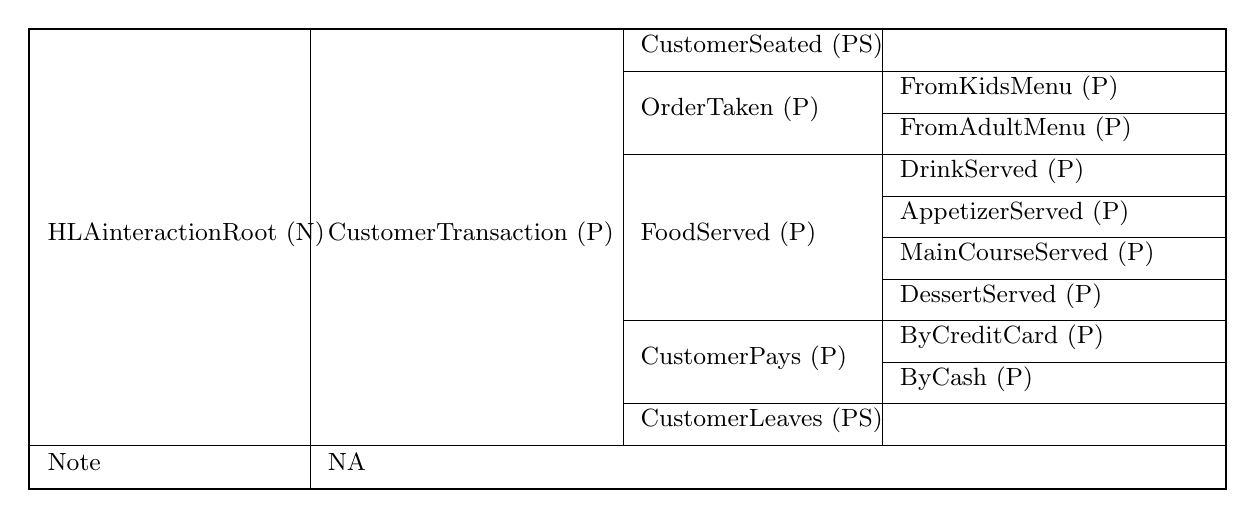
\begin{tikzpicture}[x=1pt,y=-1pt]
        \tikzset{omt7/.style={anchor=west,inner sep=0pt,font=\fontsize{9}{10}\selectfont}}
        \draw[line width=0.75pt] (0,0) rectangle (432.60,166.32);
        \draw[line width=0.28pt] (101.76,0)--(101.76,166.32);
        \draw[line width=0.28pt] (214.80,0)--(214.80,150.54);
        \draw[line width=0.28pt] (308.52,0)--(308.52,150.54);
        \draw[line width=0.28pt] (0,150.54)--(432.60,150.54);
        \draw[line width=0.28pt] (214.80,15.48)--(432.60,15.48);
        \draw[line width=0.28pt] (308.52,30.48)--(432.60,30.48);
        \draw[line width=0.28pt] (214.80,45.48)--(432.60,45.48);
        \foreach \yy in {60.54,75.54,90.54} {\draw[line width=0.28pt] (308.52,\yy)--(432.60,\yy);}
        \draw[line width=0.28pt] (214.80,105.54)--(432.60,105.54);
        \draw[line width=0.28pt] (308.52,120.54)--(432.60,120.54);
        \draw[line width=0.28pt] (214.80,135.54)--(432.60,135.54);

        \node[omt7] at (6.60,74.1) {HLAinteractionRoot (N)};
        \node[omt7] at (107.91,74.1) {CustomerTransaction (P)};
        \node[omt7] at (220.92,6.5) {CustomerSeated (PS)};
        \node[omt7] at (220.92,29.0) {OrderTaken (P)};
        \node[omt7] at (314.63,21.5) {FromKidsMenu (P)};
        \node[omt7] at (314.63,36.5) {FromAdultMenu (P)};
        \node[omt7] at (220.92,74.1) {FoodServed (P)};
        \node[omt7] at (314.63,51.6) {DrinkServed (P)};
        \node[omt7] at (314.63,66.6) {AppetizerServed (P)};
        \node[omt7] at (314.63,81.6) {MainCourseServed (P)};
        \node[omt7] at (314.63,96.6) {DessertServed (P)};
        \node[omt7] at (220.92,119.1) {CustomerPays (P)};
        \node[omt7] at (314.63,111.6) {ByCreditCard (P)};
        \node[omt7] at (314.63,126.6) {ByCash (P)};
        \node[omt7] at (220.92,141.6) {CustomerLeaves (PS)};
        \node[omt7] at (6.60,156.6) {Note};
        \node[omt7] at (107.87,156.6) {NA};
    \end{tikzpicture}%
}

\subsection{Attribute table}

\subsubsection{Purpose/background}
Each class of simulation domain objects shall be characterized by a fixed set of attribute types. These attributes are named portions of their object's state whose values can change over time (such as location or velocity of a platform). The values of HLA instance attributes are updated through the RTI and provided to other federates in a federation. Both federates and federations shall document all such object attributes in the attribute table of their SOM, FOM, and relevant SOM modules and FOM modules. The object class ``HLAobjectRoot'' shall be a superclass of all other object classes in a FOM or FOM module and in a SOM or SOM module; attributes may be assigned to it like any other object class.

Attributes of HLA object classes are specified in order to support subscription to their values by other interested members of a federation. Thus, the names of attributes and associated object classes are essential information when initializing a federation execution. Knowledge of object attributes is commonly required for effective communication between federates in a federation. In addition, although the datatypes and update policies of attributes represent characteristics that are not directly utilized by the RTI, they are important to ensuring compatibility among federates in a federation. A federate operating with very low update rates for an instance attribute could create problems for interacting federates that are operating at high update rates. The specification of datatypes and update rates in an HLA FOM is a part of the FOM ``contract'' among federates to interoperate at the specified levels. These specifications provide a common perception of the simulation space across federates in a federation, lowering the potential for inconsistency.

\subsubsection{Table format}
The attribute table of a FOM or FOM module shall describe all object attributes represented in a federation. The attribute table of a SOM or SOM module shall describe all class attributes that are published or subscribed to by the federate. The template that shall be used for the attribute table is provided by Table 8.
